%%%%%%%%%%%%%%%%%%%%%%%%%%%%%%%%%%%%%%%%%%%%%%%%%%%%%%%%%%%%%%%%%%%%%%%%%%%%%%%
%%%%%%%%%%%%%%%%%%%%%%%%%%%%%%%%%%%%%%%%%%%%%%%%%%%%%%%%%%%%%%%%%%%%%%%%%%%%%%%
\chapter{Introduction}
\label{chap:introduction}
%%%%%%%%%%%%%%%%%%%%%%%%%%%%%%%%%%%%%%%%%%%%%%%%%%%%%%%%%%%%%%%%%%%%%%%%%%%%%%%
%%%%%%%%%%%%%%%%%%%%%%%%%%%%%%%%%%%%%%%%%%%%%%%%%%%%%%%%%%%%%%%%%%%%%%%%%%%%%%%

\section{Intent}
\label{sec:intent}

The intent of this dissertation is to document my research into
\emph{formalized score control}\cite{ baca2011xi, baca2015tenor,
trevino2013compositional} in order to demonstrate a \emph{computational model
of music composition}. The term formalized score control, inspired by Iannis
Xenakis' seminal text \emph{Formalized Music}\cite{xenakis1992formalized,
baca2012}, describes the discipline of modeling and manipulating the typography
of common practice notation programmatically via software. An emphasis on
\emph{modeling}, here, is crucial. When working computationally, models provide
an explicit formal description of what objects exist within a given domain, how
they behave, and what transformations they afford. The clearer the model
becomes, the easier it is to extend and to construct increasingly higher-order
abstractions around that model. That is to say, a clear model of notation --
the description of symbols on the page -- affords a clear model of composition
-- how those symbols come to be there.

At the time of this writing, a wide variety computational models of notation
exist\cite{ baca2015tenor, trevino2013compositional, }, expressing an equally
wide range of explicitness or implicitness in their modeling, and providing
composers with varying degrees of programmatic control. For
example, many composers make use of vector graphics programs for notation,
working in a environment which behaves like a hyper-extended writing desk, but
which provides no more semantic understanding of the contents of the page than
a physical pencil does. Likewise, many composers rely on more traditional
notation software which mimics the physical page while providing some model of
common practice notation, and still others on the idiosyncratic score-modeling
systems often developed hand-in-hand with computer-assisted composition tools.

Of course it's important to understand that I don't denigrate the use of vector
graphics programs to create scores. The relative presence or absence of
notation modeling in a tool cuts both ways.

Others make use of more traditional 

- What is a notation model, what does it do, what is it good for?

- What is the name of this notational model? Abjad.

- Short history of Abjad

- An explicit model of notation affords an equally explicit model of
  composition.

- What is the name of this composition model? Consort.

- What does Consort do? Why is it interesting?


Notational and compositional modeling bring the discipline of computer science
to bear on a variety of musical questions: how does one arrange large-scale
form? what manner of rhythmic, harmonic and timbral transformations are
available? how can one describe formal structural relationships between the
objects on a page?


-   Desire to describe the process by which a score is created

-   To model the musical objects, both notational and compositional explicitly

-   Formalized score control

-   automated typesetting

-   Modern software development techniques, 

To provide a full documentation of the process of working in a formalized way,
from the low-level notational primitives through to high-level descriptions of
large-scale structure, with considerable time spent on the work in the
mid-ground, as well as proposed solutions to the practical concerns of software
development and document preparation.

Score as inseparable from the software that created

Introduce Abjad, Consort, LilyPond, Python and \LaTeX{}

Modeling acoustic music in similar ways to electronic music. How to transfer
that same facility I found in the transformations of fixed-media pieces into 
the notated domain.

Modeling is inevitably the answer: A model of notation, a model of composition.
Automated typesetting greases the wheel.

\section{Background}
\label{sec:background}

Computer-assisted composition has a fairly short history, dating at the time of
this writing a little more than half a century. While one could certainly argue
about the timeline and origins of the techniques falling under this umbrella --
and providing a complete history of computer music is not the goal of this
dissertation -- it is generally agreed that work began in earnest in the
post-war decades of the 20th century.\cite{curtis1996computer,
xenakis1992formalized} Despite its relative youth as a musical tradition,
computer-assisted composition has many practitioners and a tremendous number
of tools to work with, both generalized and idiosyncratic.

Xenakis' massed string music, Curtis Roads' granular explorations, Trevor
Wishart's schema of textural transformations.

Some of the most important tools available contemporary with my entry into the
field include OpenMusic, PWGL, Common Lisp music, and somewhat later the BACH
library for use with modern versions of Max, as well as a whole host of more
marginal experiments including LilyCollider which provides an interface between
SuperCollider -- generally used for live electronics -- and LilyPond.

My earliest experiments with computer-assisted composition involved Max/MSP,
writing patches to generate tabular data from various noise functions which I
collected into spreadsheets and painstakingly notated by hand.

Poor model - highly implicit. No automated typesetting.

That work culminated at the end of my undergraduate study in 2006 with the
never-completed score \emph{mbrsi} -- excerpted in \autoref{fig:mbrsi-score},
with spreadsheet \enquote{sources} in \autoref{fig:mbrsi-lh} and
\autoref{fig:mbrsi-rh} --, whose textural fabric of massed strings attempted to
crystallize the possibilities I felt in granular synthesis at the time: a kind
of sparkling, nervous energy hovering between a flame and the strange
Bezier-cloud outlined by starling swarms. Unfortunately, the process of simply
notating the piece by hand was gruelling, and effectively forbade any effort at
compositional exploration, let alone revising. I set it aside and spent the
next few years looking for alternative approaches to formalizing large-scale
structure in score.

\begin{figure}[H]
\begin{centering}
\includegraphics[
    page=1,
    width=\textwidth,
    height=0.9\textheight,
    keepaspectratio,
]{assets/dissertation-score-mbrsi.pdf}
\caption{The first page of \emph{mbrsi} (2006), an unfinished tablature score
for one to twelve string performers. This represents an early attempt of mine
at computationally modeling massed performers with timespans to create an
evolving \enquote{granular} texture. The instructions for the score were
created through a variety of Max/MSP patches which painstakingly converted
noise functions into text files which I then collated into spreadsheets. The
score itself was drawn by hand on size A1 graph paper with Rapidographs.
I completed seventeen of the intended fifty-three pages before stopping for the
sake of my wrists and due a general lack of faith in the project. While still
incomplete, the concerns that motivated this score remain with me.}
\label{fig:mbrsi-score}
\end{centering} 
\end{figure}

\begin{figure}[H]
\begin{centering}
\noindent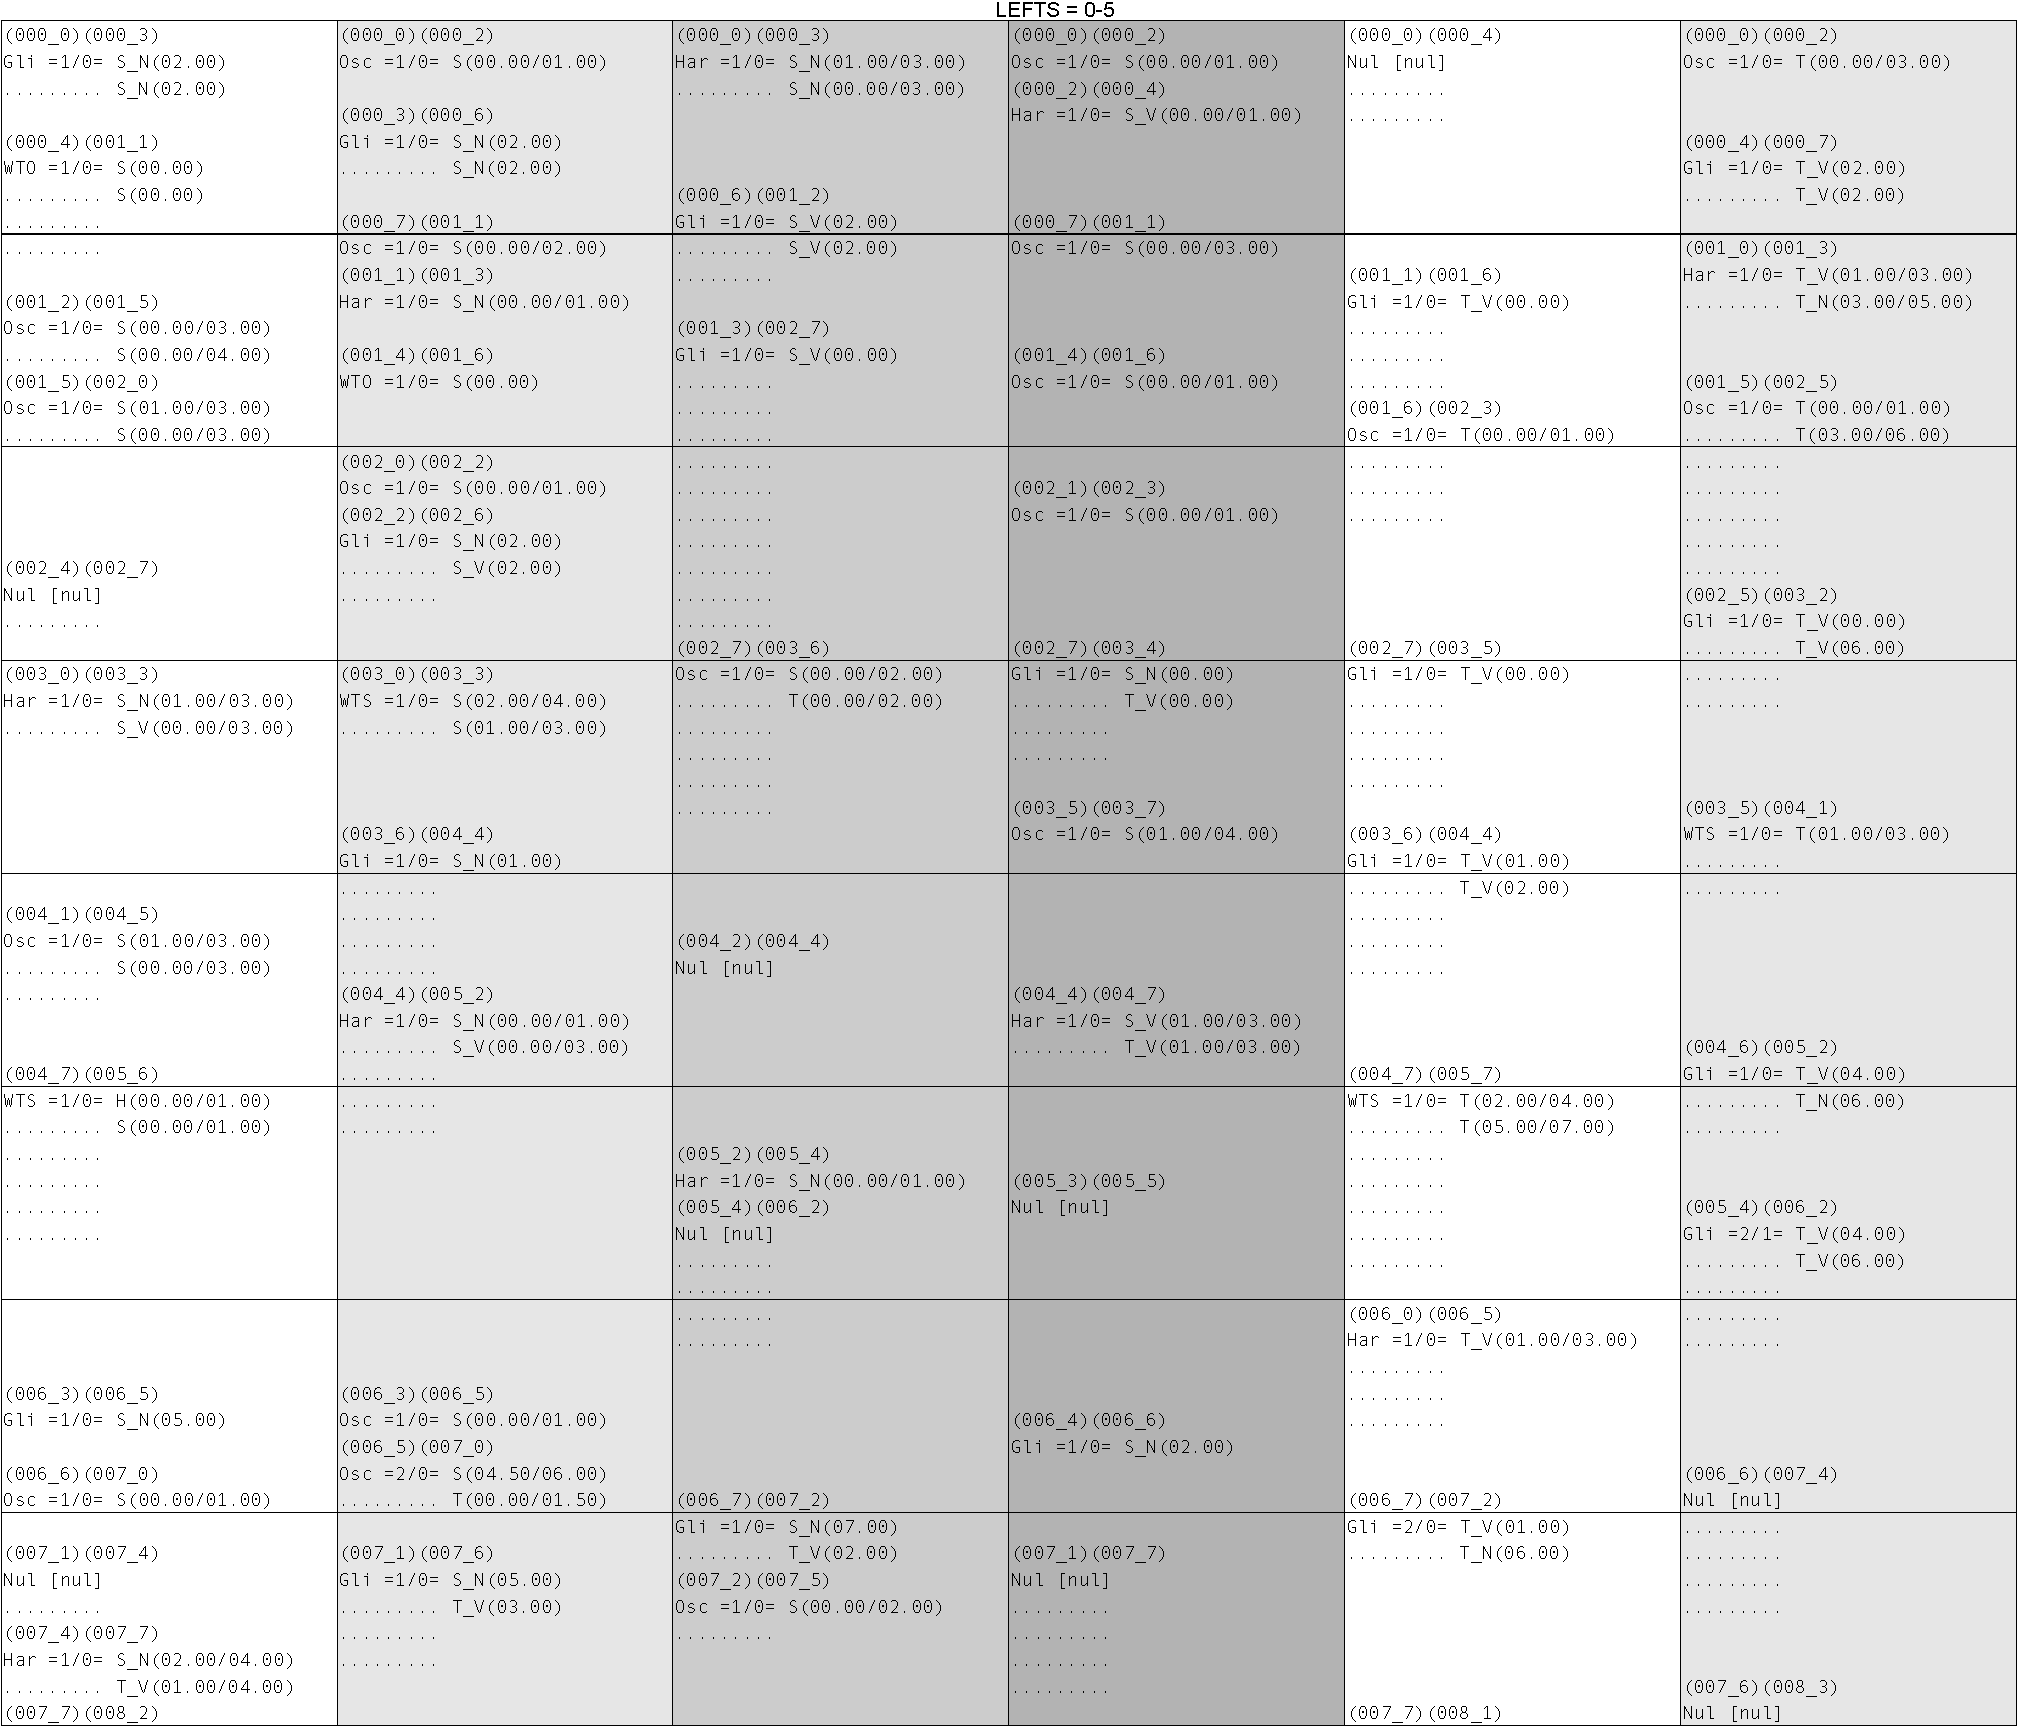
\includegraphics[
    clip=true,
    trim=0in 0in 0in 0.125in,
    page=1,
    width=\textwidth,
]{assets/dissertation-score-mbrsi-lh.pdf}
\caption{Page one of fifty-three from a spreadsheet containing fingering
instructions for six of the twelve string performers in \emph{mbrsi} (2006).}
\label{fig:mbrsi-lh}
\end{centering}
\end{figure}

\begin{figure}[H]
\begin{centering}
\noindent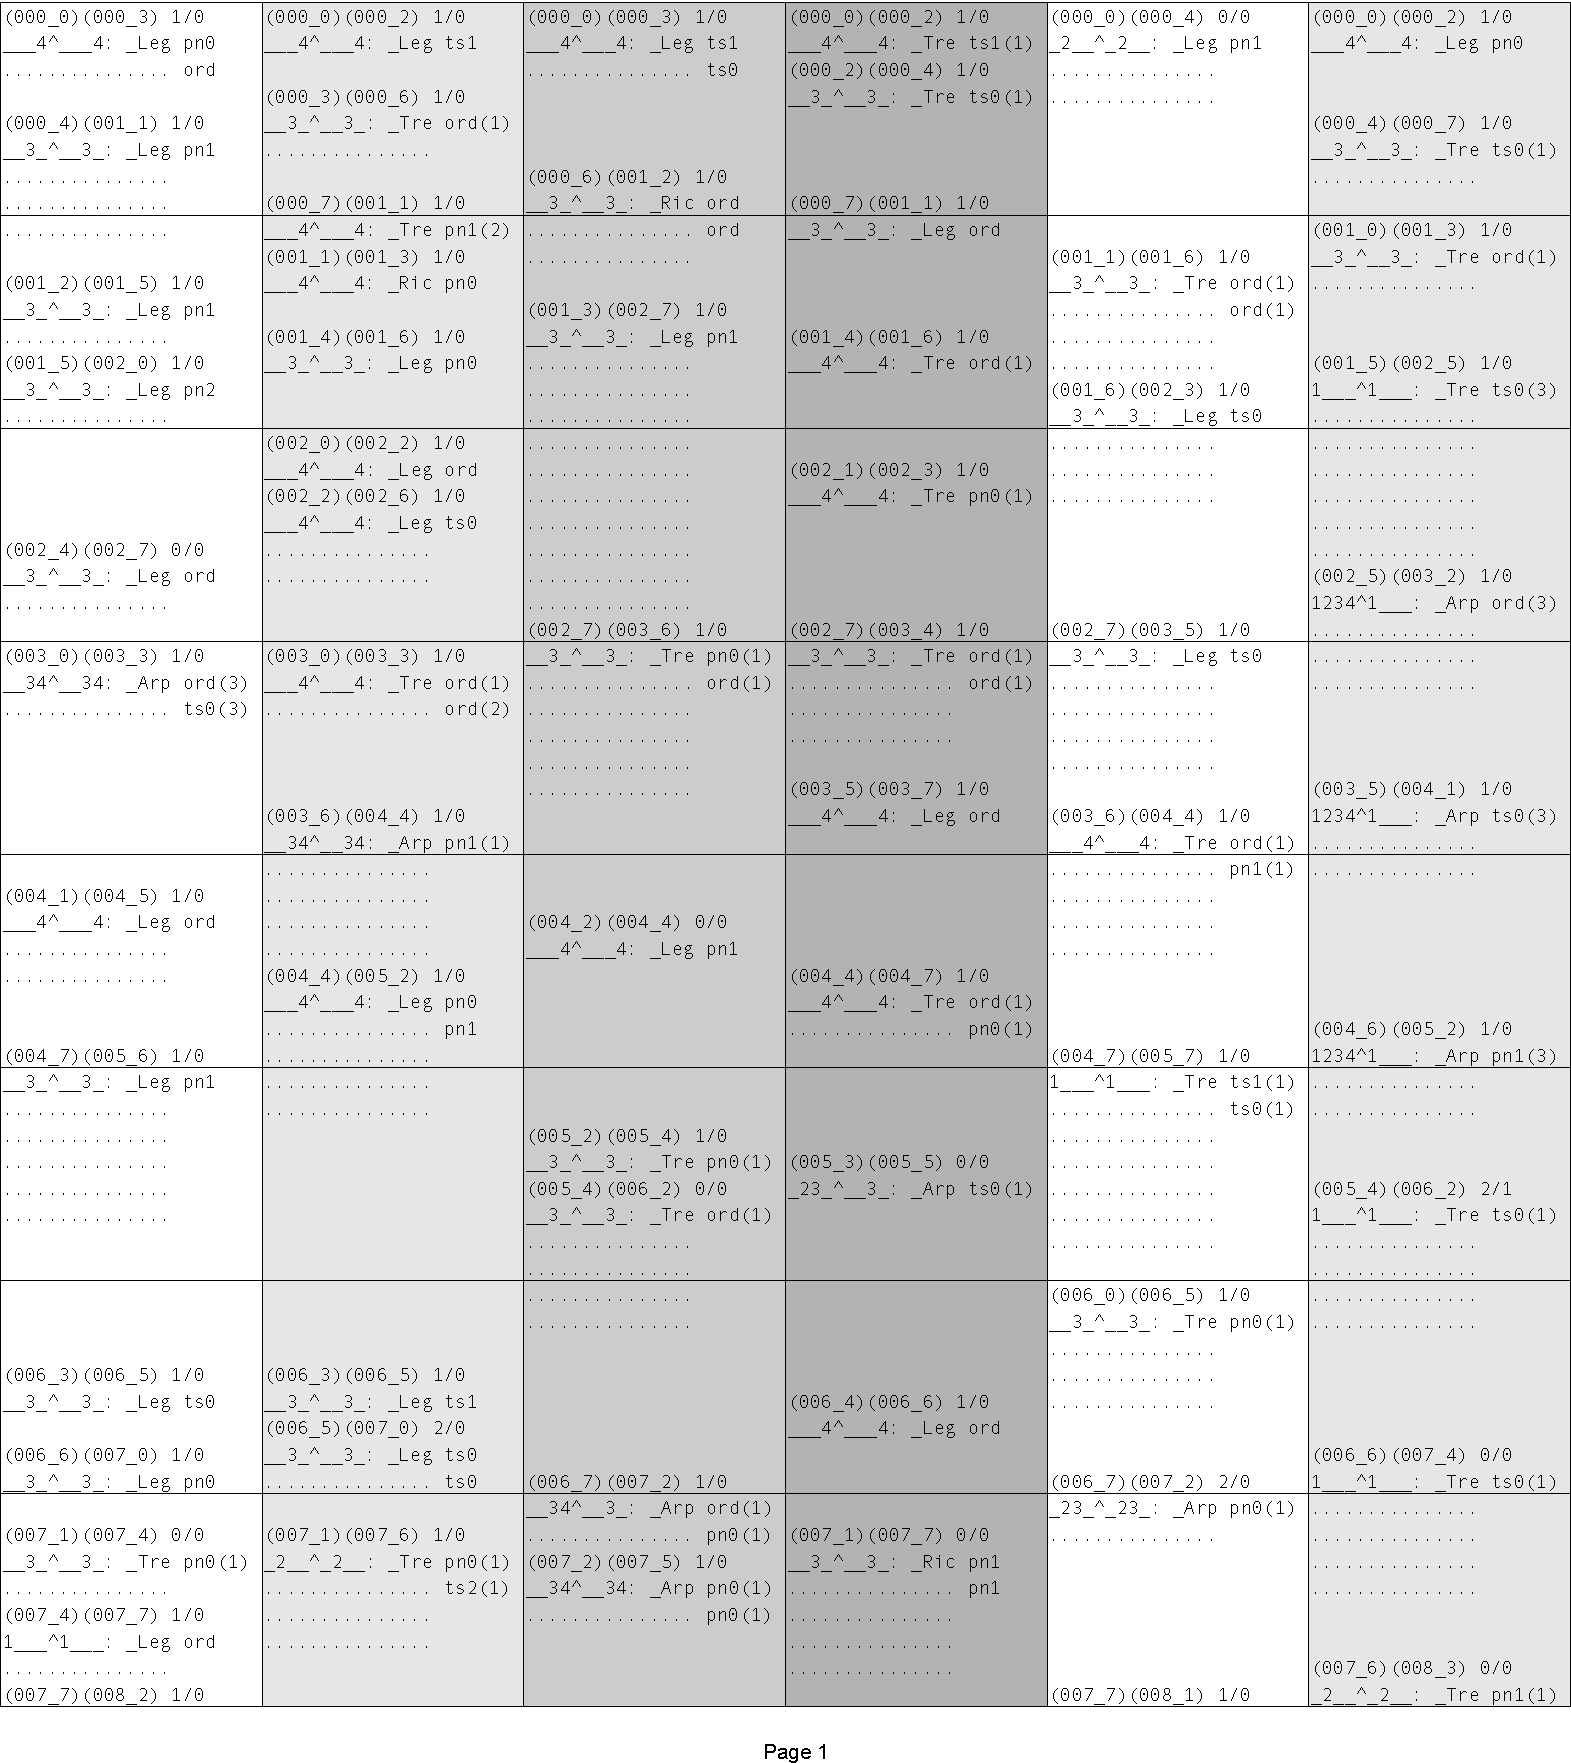
\includegraphics[
    clip=true,
    trim=0in 0.25in 0in 0in,
    page=1,
    width=\textwidth,
]{assets/dissertation-score-mbrsi-rh.pdf}
\caption{Page one of fifty-three from a spreadsheet containing bowing
instructions for six of the twelve string performers in \emph{mbrsi} (2006).}
\label{fig:mbrsi-rh}
\end{centering}
\end{figure}

A number of years later, at the beginning of my graduate studies, I was
introduced to first LilyPond, and then Abjad.

Expand on Abjad

\section{Methodology}
\label{sec:methodology}


\section{Overview of the dissertation}
\label{sec:overview-of-the-dissertation}

This dissertation consists of six chapters of prose -- including this chapter
--, followed by five chapters each presenting a score, and four extensive
appendices comprising complete code listings for the implementations of the
three most recent scores and of Consort. Please consult the source for Abjad
version 2.16\footnote{https://github.com/Abjad/abjad/releases/tag/2.16}
directly, as it is far too large to include here.

The first six chapters discuss formalized score control, gradually laying out
and building upon the concepts necessary to understand the process of modeling
notation and composition computationally. Chapter 2 presents an overview of
Abjad, detailing its structure and usage in the creation of scores. The objects
comprising Abjad's core notation model, \emph{components}, \emph{indicators}
and \emph{spanners}, are introduced, and the techniques by which those objects
are aggregated into scores, inspected, selected, iterated over, mutated,
persisted to disk, and visualized are demonstrated at length. Chapter 3 expands
on chapter 2, discussing various models of musical time implemented in Abjad,
and introducing many of tools and techniques employed in Consort to create
large-scale musical works. Timespans -- objects which model a duration of time
positioned along a timeline without regard for score hierarchy --, as well as
collections of timespans, and operations applied against both single timespans
and their collections, are presented as a means for modeling high-level
phrasing and score structure. Highly-configurable factory classes for
programmatically creating both timespan and rhythmic structures are introduced
along with a hierarchical model of meter which affords coordination between the
two models of time. Chapter 4 analyzes the mechanisms implemented in Consort's
model of composition to specify the structure of musical score at a high level
and to interpret those specifications into completely-notated segments of
music. The analysis proceeds step-by-step through the process of specification,
introducing the reader to Consort's segment-makers, music specifiers and music
settings. The discussion then turns to interpretation, divided into rhythmic-
and non-rhythmic stages. The mechanisms by which grace notes, pitches and
attachments are applied to the interpreted score are presented, providing a
link back to the iteration and selection techniques presented in chapter 2.
Chapter 5 proposes standardized solutions to practical concerns surrounding the
composition of scores in software, such as score package layout on the
file-system, typesetting workflows, version control, and testing. The means by
which an individual score segment, as described in chapter 4, is combined with
many other segments to create a complete work is presented, and the document
preparation techniques necessary for automating the extraction of parts in
LilyPond and producing the various non-musical component documents of a score
with \LaTeX{} are also introduced. Chapter 6, the conclusion to the prose
portion of the dissertation, summarizes the previously presented research,
suggests some implications and areas for improvement, and proposes directions
for future work.

The remaining chapters consist of five scores, all composed computationally
with Abjad and LilyPond, both prior to and after the development of Consort.
Chapter 7 presents \emph{Aurora} (2011), for string orchestra, which represents
the results of my first formal research into composition with timespan
structures, as well as my first formalized work which allowed multiple distinct
textures to overlap. This score implemented a very rudimentary version of the
\enquote{specify \& interpret} pattern enshrined in Consort. Chapter 8 presents
\emph{Plague Water} (2014), for baritone saxophone, electric guitar, piano and
percussion, my first attempt at composing scores in segments through explicit
specification and interpretation, and whose code-base provided Consort's
original foundation. Chapters 9, 10 and 11 present a set of pieces,
\emph{Invisible Cities (i): Zaira} (2014), for eight players, \emph{Invisible
Cities (ii): Armilla} (2015), for viola duet, and \emph{Invisible Cities (iii):
Ersilia} (2015), for chamber orchestra, all implemented via Consort. These
three scores demonstrate Consort's flexibility as tool for structuring both
large and small ensemble works of widely divergent textures, notated both
conservatively -- as in \emph{Zaira} and \emph{Ersilia} -- and more
unconventionally, with tablature -- as in Armilla.

Finally, the appendices contain the source to all classes and functions
implemented in Consort -- as of the time of this writing --, as well as the
source to all material and segment definitions, as well as any LilyPond
stylesheets, for the three Invisible Cities scores. My sincere hope is that
these appendices provide a concrete, \enquote{reverse-engineerable} even, link
between the descriptions of my research into formalized score control and the
scores written with these tools.

%\begin{markdown}
%
%# What is this?
%
%Laying out the terms.
%
%This is an analysis of a model of composition, implemented computationally.
%
%This is not an analysis of any works, although works are included.
%
%This is not a survey of techniques used by composers working in
%computer-assisted composition, but the work of one composer implementing for
%the specifics of his own process. This work may well be applicable to others in
%many ways, but I do not claim universality.
%
%Provide a description of formalized score control.
%
%Mention Abjad, Python, LilyPond and LaTeX very briefly. Drop names as
%appropriate.
%
%My aim is to provide a sufficiently detailed explanation of the theory behind
%this work as well as my specific implementation that those who read
%this would be able to consult the source to each of the three Invisible Cities
%scores included in the appendices and make some (or a lot of) sense of them.
%
%It is then, more of a tutorial than anything else, presented in order to
%explain the architectural decisions, implementations and implications behind a
%system designed to assist in the composition of music.
%
%# Background
%
%Mention Trevor Wishart's \emph{On Sonic Art} with regard to textural variation,
%and Curtis Roads' \emph{Microsound} for granular techniques.
%
%Both historical and personal.
%
%Provide wider discussion of Abjad, Python, LilyPond and LaTeX.
%
%Differentiate from Max, PWGL, OM.
%
%\end{markdown}